\documentclass[journal]{vgtc}                % final (journal style)
%\documentclass[review,journal]{vgtc}         % review (journal style)
%\documentclass[widereview]{vgtc}             % wide-spaced review
%\documentclass[preprint,journal]{vgtc}       % preprint (journal style)

%% Uncomment one of the lines above depending on where your paper is
%% in the conference process. ``review'' and ``widereview'' are for review
%% submission, ``preprint'' is for pre-publication, and the final version
%% doesn't use a specific qualifier.

%% Please use one of the ``review'' options in combination with the
%% assigned online id (see below) ONLY if your paper uses a double blind
%% review process. Some conferences, like IEEE Vis and InfoVis, have NOT
%% in the past.

%% Please note that the use of figures other than the optional teaser is not permitted on the first page
%% of the journal version.  Figures should begin on the second page and be
%% in CMYK or Grey scale format, otherwise, colour shifting may occur
%% during the printing process.  Papers submitted with figures other than the optional teaser on the
%% first page will be refused. Also, the teaser figure should only have the
%% width of the abstract as the template enforces it.

%% These few lines make a distinction between latex and pdflatex calls and they
%% bring in essential packages for graphics and font handling.
%% Note that due to the \DeclareGraphicsExtensions{} call it is no longer necessary
%% to provide the the path and extension of a graphics file:
%% 
\includegraphics{diamondrule} is completely sufficient.
%%
\ifpdf%                                % if we use pdflatex
  \pdfoutput=1\relax                   % create PDFs from pdfLaTeX
  \pdfcompresslevel=9                  % PDF Compression
  \pdfoptionpdfminorversion=7          % create PDF 1.7
  \ExecuteOptions{pdftex}
  \usepackage{graphicx}                % allow us to embed graphics files
  \DeclareGraphicsExtensions{.pdf,.png,.jpg,.jpeg} % for pdflatex we expect .pdf, .png, or .jpg files
\else%                                 % else we use pure latex
  \ExecuteOptions{dvips}
  \usepackage{graphicx}                % allow us to embed graphics files
  \DeclareGraphicsExtensions{.eps}     % for pure latex we expect eps files
\fi%

%% it is recomended to use ``\autoref{sec:bla}'' instead of ``Fig.~\ref{sec:bla}''
\graphicspath{{figures/}{pictures/}{images/}{./}} % where to search for the images

\usepackage{microtype}                 % use micro-typography (slightly more compact, better to read)
\PassOptionsToPackage{warn}{textcomp}  % to address font issues with \textrightarrow
\usepackage{textcomp}                  % use better special symbols
\usepackage{mathptmx}                  % use matching math font
\usepackage{times}                     % we use Times as the main font
\renewcommand*\ttdefault{txtt}         % a nicer typewriter font
\usepackage{cite}                      % needed to automatically sort the references
\usepackage{tabu}                      % only used for the table example
\usepackage{booktabs}                  % only used for the table example
%% We encourage the use of mathptmx for consistent usage of times font
%% throughout the proceedings. However, if you encounter conflicts
%% with other math-related packages, you may want to disable it.

%% In preprint mode you may define your own headline.
%\preprinttext{To appear in IEEE Transactions on Visualization and Computer Graphics.}

%% If you are submitting a paper to a conference for review with a double
%% blind reviewing process, please replace the value ``0'' below with your
%% OnlineID. Otherwise, you may safely leave it at ``0''.
\onlineid{0}

%% declare the category of your paper, only shown in review mode
\vgtccategory{Research}
%% please declare the paper type of your paper to help reviewers, only shown in review mode
%% choices:
%% * algorithm/technique
%% * application/design study
%% * evaluation
%% * system
%% * theory/model
\vgtcpapertype{please specify}

%% Paper title.
\title{Visualizing Spatio-Temporal Data with Dynamic Cartogram}

%% This is how authors are specified in the journal style

%% indicate IEEE Member or Student Member in form indicated below
\author{Yiren Ding and Di Zhong}
\authorfooter{
%% insert punctuation at end of each item
\item
 Yiren Ding is with Northeastern University. E-mail: ding.yir@husky.neu.edu.
\item
 Di Zhong is with Northeastern University. E-mail: dizhong@ccs.neu.edu.
}

%other entries to be set up for journal
\shortauthortitle{Biv \MakeLowercase{\textit{et al.}}: Interactive Cartogram}
%\shortauthortitle{Firstauthor \MakeLowercase{\textit{et al.}}: Paper Title}

%% Abstract section.

\abstract{summarize map, map with dots, etc... and pitch the tool as easy to visualize change of data in time in terms of the geological density.
} % end of abstract

%% Keywords that describe your work. Will show as 'Index Terms' in journal
%% please capitalize first letter and insert punctuation after last keyword
\keywords{map, cartogram, trend}

%% ACM Computing Classification System (CCS). 
%% See <http://www.acm.org/class/1998/> for details.
%% The ``\CCScat'' command takes four arguments.

\CCScatlist{ % not used in journal version
 \CCScat{K.6.1}{Management of Computing and Information Systems}%
{Project and People Management}{Life Cycle};
 \CCScat{K.7.m}{The Computing Profession}{Miscellaneous}{Ethics}
}

%% Uncomment below to include a teaser figure.
\teaser{
  \centering
  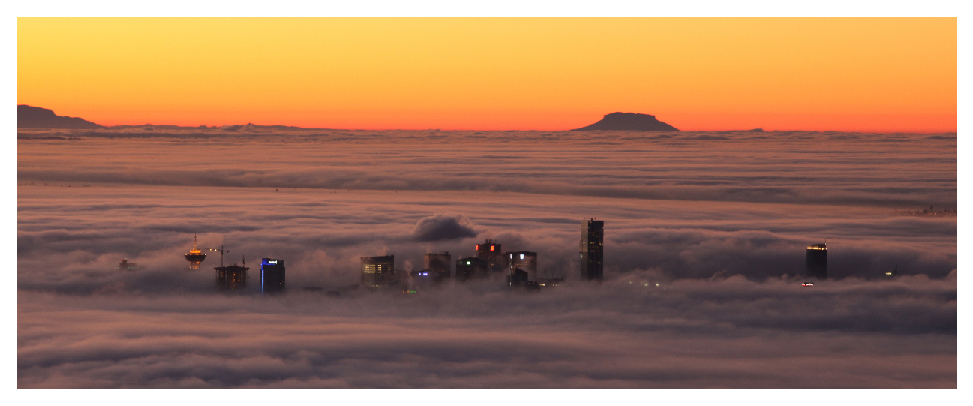
\includegraphics[width=\linewidth]{CypressView}
  \caption{A screenshot of the tool}
	\label{fig:teaser}
}

%% Uncomment below to disable the manuscript note
%\renewcommand{\manuscriptnotetxt}{}

%% Copyright space is enabled by default as required by guidelines.
%% It is disabled by the 'review' option or via the following command:
% \nocopyrightspace

\vgtcinsertpkg

%%%%%%%%%%%%%%%%%%%%%%%%%%%%%%%%%%%%%%%%%%%%%%%%%%%%%%%%%%%%%%%%
%%%%%%%%%%%%%%%%%%%%%% START OF THE PAPER %%%%%%%%%%%%%%%%%%%%%%
%%%%%%%%%%%%%%%%%%%%%%%%%%%%%%%%%%%%%%%%%%%%%%%%%%%%%%%%%%%%%%%%%

\begin{document}

%% The ``\maketitle'' command must be the first command after the
%% ``\begin{document}'' command. It prepares and prints the title block.

%% the only exception to this rule is the \firstsection command
\firstsection{Introduction}

\maketitle

%% \section{Introduction} %for journal use above \firstsection{..} instead
More detailed form of abstract. 

Introduce the tool, the kinds of graph it provides, and the reasoning of layout for each view.

\section{Related Works}

\begin{itemize}

\item start from introducing about the origin of maps

\item go towards having data points labeled on maps, for example during wars

\item Tobler, Waldo (March 2004). "Thirty-Five Years of Computer Cartograms". Annals of the Association of American Geographers.
\begin{itemize}
\item evolve of cartograms
\item types of cartograms
\item how it goes beyond that, and active research
\end{itemize}
\item Effectiveness of Cartogram for the Representation of Spatial Data

\item Value-by-alpha Maps: An Alternative Technique to the Cartogram, talk about other alternative choices

\end{itemize}

\section{Process}
\begin{itemize}
\item interviews
\begin{itemize}
\item why we chose to interview the people we interview
\item remember to refer to names and title
\end{itemize}
\item Task 1
\begin{itemize}
\item Check how the amount of tweets changed during St Patrick's day.
\item The most important feature of our visualization is that the dynamic cartogram. Users can drag the button on time axis, the cartogram will change to visualize corronsond data  with animation.  Users are able to observe trend easily. Also, it will be a beautiful and readily comprehensible way to do presentation.
\item Our tool also provide an option that visualize the data in small multiples. Users can add several time stamp and view cartogram for each time stamp in another tab. This is useful when user want to check the trend in a specific time interval. 
We also provide traditional line chart, users are able to check trend of data from line chart
\end{itemize}
\item Task 2
\begin{itemize}
\item How football fan’s emotion changed after a score during a match. Do they have correlation?
\item In cartogram, color and shape distortion can represent two attributes. So we plan to use shape distortion represent the number of tweets and color to represent the emotion of those tweets. And the map itself represent another attributes- location. So our visualization can encoding above three attributes at the same time, which is difficult to do in other visualizations. 
\end{itemize}

\item Task 5
\begin{itemize}
\item Is there any area in which St Patrick's day more popular?
\item In cartogram, we can use shape distortion and color to encoding the same attributes, this redundant visualization( Most significant distorted state, and the highest color saturation) helps user locate maximum/minimum value in data easier.
\end{itemize}

\item Task 3
\begin{itemize}
\item What is the distribution of tweets amount for each state?
\item One of the most common task is to check the distribution of data. We provide standard bar chart that (with x-axis is states, and y-axis is an attributes ) that allow user to do this task in our application. 
\end{itemize}
\item Task 4
\begin{itemize}
\item Where and When is the peak of celebration in St Patrick's day. 
\item To check where and when is the peak of celebration in St.Patrick's day, users can check the line chart of data. It shows the trend of data, also it is easy to find peaks in line chart. Users can also browse by dragging time button in cartrogram. It is more useful in presentation.
\end{itemize}
\item Task 6
\begin{itemize}
\item Compare the popularity of St Patrick's day in California and New York
\item Users are allowed to add filters to data. After applying proper filter, users can compare data in two or several states in a certain time stamp or the sum of tweets. 
\end{itemize}
\end{itemize}

\section{Design}
\begin{itemize}
\item at first the website show an entrying page that says the name of the project and authors
\item First Page is the main view
\begin{itemize}
\item cartogram itself takes up most of the space
\item left slide bar shows the loaded data
\item right slide bar shows an extra bar graph, for detailed data
\item choice to select colors
\end{itemize}
\item Second page shows small multiples from data points that the user select, and trendline graph.
\begin{itemize}
\item able to choose to delete small multiple
\item able to see the exact trend change from the precise graph
\item choice to select colors
\end{itemize}
\end{itemize}

\section{Discussion}
\begin{itemize}
\item how's the usability of the project?
\item difficulties in implementation?
\item did we have to give up any original design thought to make the project more doable?
\end{itemize}

\section{Conclusion}
\begin{itemize}
\item draw some conclusion from discussion
\item summarize about the good parts
\begin{itemize}
\item how did it correspond to our task? were out task goals realistic? how much did they help?
\item any surprise good parts?
\end{itemize}
\item summarize about what we could improve, change, or have done better
\begin{itemize}
\item how could we have designed the interview process to make task analysis more helpful?
\item what other part did we not think about?
\end{itemize}
\end{itemize}

\section{References}

\begin{itemize}

\item Tobler, Waldo (March 2004). "Thirty-Five Years of Computer Cartograms". Annals of the Association of American Geographers.
\item Effectiveness of Cartogram for the Representation of Spatial Data

\item Value-by-alpha Maps: An Alternative Technique to the Cartogram, talk about other alternative choices

\item more?

\end{itemize}


%% if specified like this the section will be committed in review mode
\acknowledgments{
The authors wish to thank A, B, and C. This work was supported in part by
a grant from XYZ (\# 12345-67890).}

%\bibliographystyle{abbrv}
\bibliographystyle{abbrv-doi}
%\bibliographystyle{abbrv-doi-narrow}
%\bibliographystyle{abbrv-doi-hyperref}
%\bibliographystyle{abbrv-doi-hyperref-narrow}

\bibliography{template}
\end{document}

